%This is my super simple Real Analysis Homework template

\documentclass{article}
\usepackage[utf8]{inputenc}
\usepackage[english]{babel}
\usepackage{amsmath,bm}
\usepackage{minted}
\usepackage[]{tcolorbox}
\usepackage[]{amsthm} %lets us use \begin{proof}
\usepackage[]{amssymb} %gives us the character \varnothing
\DeclareMathOperator{\sech}{sech}

\title{Homework 1}
\author{Guilherme Albertini}
\date\today
%This information doesn't actually show up on your document unless you use the maketitle command below

\begin{document}
\maketitle %This command prints the title based on information entered above

%Section and subsection automatically number unless you put the asterisk next to them.
\section*{Theory}
Let $Linear_1 \rightarrow f \rightarrow  Linear_2 \rightarrow g $ be a be a
two-layer neural net architecture whereby $Linear_i(x) =
  \bm{W}^{(i)}\bm{x}+\bm{b}^{(i)}$ is the $i^{th}$ affine transformation and
$f,
  g$ are element-wise nonlinear activation functions (else must use transposes
and/or Hadamard products). When an input $\bm{x}\in
  \mathbb{R}^n$ is fed into the network, $\bm{\hat{y}} \in \mathbb{R}^K$ is
obtained as output.
%Basically, you type whatever text you want and use the $ sign to enter "math mode".
%For fancy calligraphy letters, use \mathcal{}
%Special characters are their own commands

\subsection*{Problem 1: Regression Task}
We would like to perform regression task. We choose
$f(\cdot)=5(\cdot)^{+}=5ReLU(\cdot)$ and $g$ to be the identity function. To
train, we choose MSE loss function,
$\ell_{MSE}(\bm{\hat{y}},\bm{y})=||(\bm{\hat{y}}-\bm{y})||^2$.
\begin{enumerate}
  \item Name and mathematically describe the 5 programming steps you
        would take to train this model with PyTorch using SGD on a single batch
        of data.
        \begin{tcolorbox}
          \begin{enumerate}
            \item First compute a prediction from the model (the forward pass);
                  $\tilde{y}=model(x)$
            \item Second compute the loss through computation of the energy
            \item Zero the gradient parameters; $optimiser.zero\_grad()$
            \item Compute and accumulate gradient parameters; $L.backward()$
            \item Finally step in the opposite direction of the gradient;
                  $optimiser.step()$
          \end{enumerate}
        \end{tcolorbox}
  \item For a single data point $(x,y)$, write down all inputs and outputs for
        forward pass of each layer. You can only use variables and mechanics
        specified
        prior in your answer.
        \begin{table}[]
          \begin{tcolorbox}
            \centering
            \begin{tabular}{|c|c|l|cc}
              \cline{1-3}
              \textbf{Layer}                                  & \textbf{Input} & \textbf{Output} &  & \\
              \cline{1-3}
              \textit{$Linear_1$}                             & $\bm{x}$       &
              $\bm{z_1}=\bm{W}^{(1)}\bm{x}+\bm{b}^{(1)}$      &                &                      \\ \cline{1-3}
              \textit{f}                                      & $\bm{z_1}$     &
              $\bm{z_2}=5(\bm{W}^{(1)}\bm{x}+\bm{b}^{(1)})^+$ &                &                      \\
              \cline{1-3}
              \textit{$Linear_2$}                             & $\bm{z_2}$     &
              $\bm{z_3}=5\bm{W}^{(2)}(\bm{W}^{(1)}\bm{x}+\bm{b}^{(1)})^++\bm{b}^{(2)}$
                                                              &                &                      \\ \cline{1-3}
              \textit{g}                                      & $\bm{z_3}$     & $\bm{z_3}$
                                                              &                &                      \\ \cline{1-3}
              \textit{Loss}                                   & $\bm{z_3, y}$  &
              $||\bm{\hat{y}-y}||^2=||5\bm{W}^{(2)}(\bm{W}^{(1)}\bm{x}+\bm{b}^{(1)})^++\bm{b}^{(2)}-\bm{y}||^2$
                                                              &                &                      \\ \cline{1-3}
            \end{tabular}
          \end{tcolorbox}
        \end{table}

  \item Write down the gradients calculated from the backward pass. You can
        only use the following variables: $\bm{x,y,W^{(1)},b^{(1)},W^{(2)},b^{(2)}},
          \frac{\partial \ell}{\partial \bm{\hat{y}}}, \frac{\partial \bm{z_2}}{\partial
            \bm{z_1}},\frac{\partial \bm{\hat{y}}}{\partial \bm{z_3}}$, where
        $\bm{z_1,z_2,z_3,\hat{y}}$ are outputs of $Linear_1,f,Linear_2,g$,
        respectively.
        \begin{tcolorbox}
          Dimensions shown are used throughout ($z_1,z_2 \in \mathbb{R}^h$):
          \begin{flalign*}
            x                                      & \in \mathbb{R}^n           \\
            \hat{y}                                & \in \mathbb{R}^K           \\
            \ell                                & \in \mathbb{R} \\
            W^{(1)}                                & \in \mathbb{R}^{h\times n} \\
            b^{(1)}                                & \in \mathbb{R}^{h}         \\
            W^{(2)}                                & \in \mathbb{R}^{K\times h} \\
            b^{(2)}                                & \in \mathbb{R}^{K}         \\
            \frac{\partial \ell}{\partial W^{(1)}} & \in \mathbb{R}^{n\times h} \\
            \frac{\partial \ell}{\partial b^{(1)}} & \in \mathbb{R}^{1\times h} \\
            \frac{\partial \ell}{\partial W^{(2)}} & \in \mathbb{R}^{h\times K} \\
            \frac{\partial \ell}{\partial b^{(2)}} & \in \mathbb{R}^{1\times K} \\
            \frac{\partial \ell}{\partial \hat{y}} & \in \mathbb{R}^{1\times K} \\
            \frac{\partial \hat{y}}{\partial z_3} & \in \mathbb{R}^{K\times K} \\
            \frac{\partial z_3}{\partial z_2} & \in \mathbb{R}^{K\times h}\\
            \frac{\partial z_2}{\partial z_1} & \in \mathbb{R}^{h\times h}\\
            \frac{\partial z_1}{\partial b_1} & \in \mathbb{R}^{h\times h}\\
            \frac{\partial z_1}{\partial W^{(1)}} & \in \mathbb{R}^{h \times (h \times n)}\\
            \frac{\partial z_3}{\partial b^{(2)}} & \in \mathbb{R}^{K \times K}\\
            \frac{\partial z_3}{\partial b^{(2)}} & \in \mathbb{R}^{K \times K}\\
            \frac{\partial z_3}{\partial W^{(2)}} & \in \mathbb{R}^{K \times (K \times h)}
          \end{flalign*}
        \end{tcolorbox}
        \begin{tcolorbox}

          \begin{flalign*}
            \frac{\partial \ell}{\partial z_3} &= \frac{\partial \ell}{\partial \hat{y}}\frac{\partial \hat{y}}{\partial z_3}\\
            \frac{\partial \ell}{\partial z_1} &= \frac{\partial \ell}{\partial \hat{y}}\frac{\partial \hat{y}}{\partial z_3}\frac{\partial z_3}{\partial z_2}\frac{\partial z_2}{\partial z_1}=\frac{\partial \ell}{\partial \hat{y}}\frac{\partial \hat{y}}{\partial z_3}W^{(2)}\frac{\partial z_2}{\partial z_1}\\
            \frac{\partial \bm{\ell}}{\partial \bm{b^{(2)}}}   & = \frac{\partial
              \bm{\ell}}{\partial \bm{\hat{y}}}\frac{\partial \bm{\hat{y}}}{\partial
            \bm{z_3}}\frac{\partial \bm{z_3}}{\partial \bm{b^{(2)}}}                                                              \\
                                                               & =\frac{\partial \bm{\ell}}{\partial \bm{\hat{y}}}\frac{\partial
            \bm{\hat{y}}}{\partial \bm{z_3}}\\ 
            \frac{\partial \ell}{\partial b^{(1)}} &= \frac{\partial \ell}{\partial \hat{y}}\frac{\partial \hat{y}}{\partial z_3}W^{(2)}\frac{\partial z_2 }{\partial z_1} \\ 
            \frac{\partial \ell}{\partial W^{(1)}} = \frac{\partial \ell}{\partial z_1} \frac{\partial z_1}{\partial W^{(1)}} &= \sum_i \frac{\partial \ell}{\partial (z_1)_i}\frac{\partial (z_1)_i}{\partial W^{(1)}} = \frac{\partial \ell}{\partial z_1}x^T = x\frac{\partial \ell}{\partial z_1}\\
            &= x\frac{\partial \ell}{\partial \hat{y}}\frac{\partial \hat{y}}{\partial z_3}W^{(2)}\frac{\partial z_2}{\partial z_1} \\
            \frac{\partial \ell}{\partial W^{(2)}} = \frac{\partial \ell}{\partial z_3} \frac{\partial z_3}{\partial W^{(2)}} &= \sum_i \frac{\partial \ell}{\partial (z_3)_i}\frac{\partial (z_3)_i}{\partial W^{(2)}} = \frac{\partial \ell}{\partial z_3}{z_2}^T =  z_2\frac{\partial \ell}{\partial z_3}\\
            &=5(\bm{W}^{(1)}\bm{x}+\bm{b}^{(1)})^+\frac{\partial \ell}{\partial \hat{y}}\frac{\partial \hat{y}}{\partial z_3}\\                                    
          \end{flalign*}
        \end{tcolorbox}
  \item Show the elements of $\frac{\partial \bm{z_2}}{\partial \bm{z_1}},
          \frac{\partial \bm{\hat{y}}}{\partial \bm{z_3}},\frac{\partial \ell}{\partial
            \bm{\hat{y}}}$. Be careful about dimensionality.
        \begin{tcolorbox}
          \begin{flalign*}                                        
            \left( \frac{\partial \bm{z_2}}{\partial \bm{z_1}}	\right)_{ii} & =
            \begin{cases} 0,                            & z_{1i} < 0 \\ 5, & z_{1i} > 0 \\ \text{undefined (or
              assigned a value 0)}, & z_{1i} = 0\end{cases}                                            \\
            &\text{Note: the above is a diagonal matrix}                                                                                                      \\
            \left(\frac{\partial \bm{\hat{y}}}{\partial \bm{z_3}}
            \right)_{ii}                                                   & = 1 \text{ (and 0 elsewhere, off of diagonal; an identity
            matrix)}                                                                                                                   \\
            \frac{\partial \ell}{\partial \bm{\hat{y}}}                    & = \frac{\partial
              (||\bm{\hat{y}-y||^2})}{\partial \bm{\hat{y}}}=2\bm{{(\hat{y}-y)}^T} \text{ (A
            vector)}\\
            & \implies 2(\hat{y}-y)_i \text{ are the elements}
          \end{flalign*}
        \end{tcolorbox}

\end{enumerate}

%If you want centered math on its own line, you can use a slash and square
%bracket.\\
%\[
%  \left \{
%  \sum\limits_{k=1}^\infty l(I_k):A\subseteq \bigcup_{k=1}^\infty \{I_k\}
%  \right \}
%\]
%The left and right commands make the brackets get as big as we need them to
%be.

\clearpage %Gives us a page break before the next section. Optional.
\subsection*{Problem 2: Classification Task}
We would like to perform multi-class classification task, so we set $f = \tanh$
and $g = \sigma$, the logistic sigmoid function,
$\sigma(z)=\frac{1}{1+\exp(-z)}$.
\begin{enumerate}
  \item If you want to train this network, what do you need to change in the
        equations of (1.2), (1.3) and (1.4), assuming we are using the same MSE loss
        function. Consult updated chart above.
        \begin{table}[]
          \begin{tcolorbox}
            \centering
            \begin{tabular}{|c|c|l|cc}
              \cline{1-3}
              \textbf{Layer}                                  & \textbf{Input} & \textbf{Output} &  & \\
              \cline{1-3}
              \textit{$Linear_1$}                             & $\bm{x}$       &
              $\bm{z_1}=\bm{W}^{(1)}\bm{x}+\bm{b}^{(1)}$      &                &                      \\ \cline{1-3}
              \textit{f}                                      & $\bm{z_1}$     &
              $\bm{z_2}=\tanh(\bm{W}^{(1)}\bm{x}+\bm{b}^{(1)})$ &                &                      \\
              \cline{1-3}
              \textit{$Linear_2$}                             & $\bm{z_2}$     &
              $\bm{z_3}=\bm{W}^{(2)}\tanh(\bm{W}^{(1)}\bm{x}+\bm{b}^{(1)})+\bm{b}^{(2)}$
                                                              &                &                      \\ \cline{1-3}
              \textit{g}                                      & $\bm{z_3}$     & $\sigma(z_3)=\bm{\frac{1}{1+\exp(-z_3)}}$
                                                              &                &                      \\ \cline{1-3}
              \textit{Loss}                                   & $\bm{\hat{y}=\sigma(z_3), y}$  &
              $||\bm{\hat{y}-y}||^2=||\bm{\sigma(z_3)}-\bm{y}||^2$
                                                              &                &                      \\ \cline{1-3}
            \end{tabular}
          \end{tcolorbox}
        \end{table}
        
        \begin{tcolorbox}
          \begin{flalign*}
            \frac{\partial \ell}{\partial z_3} &= \frac{\partial \ell}{\partial \hat{y}}\frac{\partial \hat{y}}{\partial z_3}\\
            \frac{\partial \ell}{\partial z_1} &= \frac{\partial \ell}{\partial \hat{y}}\frac{\partial \hat{y}}{\partial z_3}\frac{\partial z_3}{\partial z_2}\frac{\partial z_2}{\partial z_1}=\frac{\partial \ell}{\partial \hat{y}}\frac{\partial \hat{y}}{\partial z_3}W^{(2)}\frac{\partial z_2}{\partial z_1}\\
            \frac{\partial \bm{\ell}}{\partial \bm{b^{(2)}}}   & = \frac{\partial
              \bm{\ell}}{\partial \bm{\hat{y}}}\frac{\partial \bm{\hat{y}}}{\partial
            \bm{z_3}}\frac{\partial \bm{z_3}}{\partial \bm{b^{(2)}}}                                                              \\
                                                               & =\frac{\partial \bm{\ell}}{\partial \bm{\hat{y}}}\frac{\partial
            \bm{\hat{y}}}{\partial \bm{z_3}} \\ 
            \frac{\partial \ell}{\partial b^{(1)}} &= \frac{\partial \ell}{\partial z_1}\frac{\partial z_1}{\partial b^{(1)}} = \frac{\partial \ell}{\partial \hat{y}}\frac{\partial \hat{y}}{\partial z_3}W^{(2)}\frac{\partial z_2}{\partial z_1}\\ 
            \frac{\partial \ell}{\partial W^{(1)}} = \frac{\partial \ell}{\partial z_1} \frac{\partial z_1}{\partial W^{(1)}} &= \sum_i \frac{\partial \ell}{\partial (z_1)_i}\frac{\partial (z_1)_i}{\partial W^{(1)}} = \frac{\partial \ell}{\partial z_1}x^T\\
            &=x\frac{\partial \ell}{\partial \hat{y}}\frac{\partial \hat{y}}{\partial z_3}W^{(2)}\frac{\partial z_2}{\partial z_1} \\
            \frac{\partial \ell}{\partial W^{(2)}} = \frac{\partial \ell}{\partial z_3} \frac{\partial z_3}{\partial W^{(2)}} &= \sum_i \frac{\partial \ell}{\partial (z_3)_i}\frac{\partial (z_3)_i}{\partial W^{(2)}} = \frac{\partial \ell}{\partial z_3}{z_2}^T\\
            &=\tanh(\bm{W}^{(1)}\bm{x}+\bm{b}^{(1)})\frac{\partial \ell}{\partial \hat{y}}\frac{\partial \hat{y}}{\partial z_3}\\
            {\left(\frac{\partial z_2}{\partial z_1}  \right)}_{ii} = [{(\sech(\bm{W}^{(1)}\bm{x}+\bm{b}^{(1)}))}]^2_{1i} &\text{ and off diagonal elements are 0}\\
            {\left(\frac{\partial \hat{y}}{\partial z_3}  \right)}_{ii} = \sigma((z_3)_i)(1-\sigma(z_3)_i) &\text{ and off diagonal elements are 0}\\
            \frac{\partial \ell}{\partial \bm{\hat{y}}}                    & = \frac{\partial
              (||\bm{\hat{y}-y||^2})}{\partial \bm{\hat{y}}}=2\bm{{(\hat{y}-y)}^T}\\
            & \implies 2(\hat{y}-y)_i \text{ are the elements}
          \end{flalign*}
        \end{tcolorbox}
        
  \item Now you think you can do a better job by using a Binary Cross Entropy
        (BCE) loss function
        $\ell_{BCE}(\bm{\hat{y},y})=\frac{1}{K}\sum_{i=1}^{K}-[y_i\log(\hat{y_i})+(1-y_i)\log(1-\hat{\hat{y_i}})]$.
        What needs to change from the previous?
        \begin{tcolorbox}
          |Loss|\\
          Input: $\bm{\hat{y}}$\\
          Output:
          $\ell_{BCE}(\bm{\hat{y},y})=\frac{1}{K}\sum_{i=1}^{K}-[y_i\log(\hat{y_i})+(1-y_i)\log(1-\hat{y_i})],$\\
          $\hat{y_i}=\frac{1}{1+\exp(-z_{3i})}$\\
          $\frac{\partial \ell}{\partial
              \hat{y}}=\frac{1}{K}(\frac{-y}{\hat{y}}+\frac{1-y}{1-\hat{y}})^T\implies \frac{1}{K}\frac{\hat{y_i}-y_i}{\hat{y_i}(1-\hat{y_i})}$ \text{ are elements}
        \end{tcolorbox}
  \item Things are getting better. You realize that not all intermediate hidden
        activations need to be binary (or soft version of binary). You decide to use
        $f(\cdot)=(\cdot)^{+}$ but keep g as $\sigma$. Explain why this choice of f can
        be beneficial for training a (deeper) network.
        \begin{tcolorbox}
          Sigmoid function is more computationally intensive to compute compared
          to ReLU due to exponential operation; the latter produces sparsity in matrices
          which encourages numerical optimization techniques taking advantage of this
          time and space complexity reduction.
        \end{tcolorbox}
        \begin{tcolorbox}
          ReLU also avoids the vanishing gradient problem, whereby the number of
          parameters receive very small updates such that the nodes deviate greatly from
          their optimal value. As the gradient is constant for ReLU compared to the
          sigmoid gradient always being smaller than 1, successive operations will start
          to prohibit learning.
        \end{tcolorbox}
\end{enumerate}

\subsection*{Problem 3: Conceptual Questions}
%
\begin{enumerate}
  \item Why is softmax actually softargmax?
        \begin{tcolorbox}
          The "softmax" is not a smooth approximation to the maximum function -- it
          is actually an approximation to the arg max function whose value is the index
          that has the maximum. Accordingly, some prefer the "softargmax" terminolgy to
          emphasize this distinction.
        \end{tcolorbox}
  \item Draw the computational graph defined by this function, with inputs $x,
          y, z \in \mathbb{R}$ and output $w \in \mathbb{R}$. You make use symbols $x, y,
          z,w$, and operators $+,\star$ in your solution. Be sure to use the correct
        shape for symbols and
        operators as shown in class.
        \begin{enumerate}
          \item $a = x \star y + z  $
          \item $b = (x+x) \star a$
          \item $w = a \star b$
        \end{enumerate}
        \includegraphics[width=15cm]{"diagram.jpg"}
  \item Draw the graph of the following (and its derivative):
        \begin{enumerate}
          \item ReLU()
                \begin{tcolorbox}
                  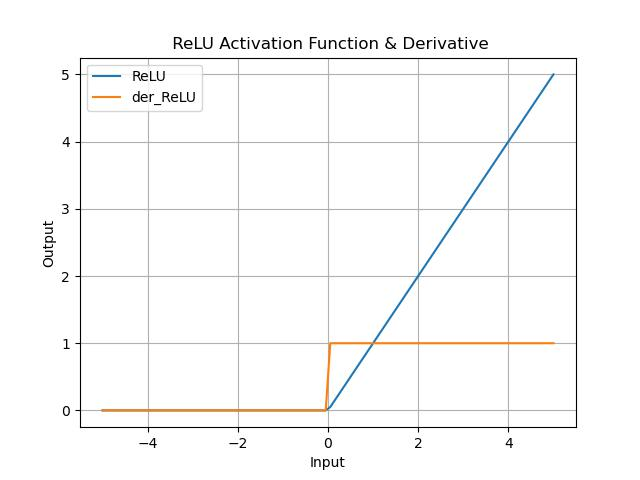
\includegraphics[width=9.5cm]{relu.jpg}
                \end{tcolorbox}
                \begin{minted}[]{python}
def ReLU(x):
  data = [max(0, value) for value in x]
  return np.array(data, dtype=float)
def der_ReLU(x):
  data = [1 if value>0 else 0 for value in x]
  return np.array(data, dtype=float)
                \end{minted}
          \item LeakyReLU(neg slope is 0.01)
                \begin{tcolorbox}
                  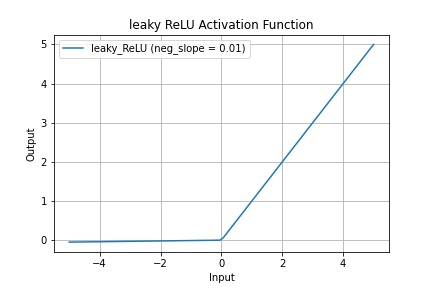
\includegraphics[width=9.5cm]{leaky_relu.jpg}
                \end{tcolorbox}
                \begin{minted}[]{python}
def leaky_ReLU(x, slope):
    data = [max(slope*value, value) for value in x]
    return np.array(data, dtype=float)  
def der_leaky_ReLU(x, slope):
    data = [1 if value>0 else slope for value in x]
    return np.array(data, dtype=float)                
                \end{minted}
          \item Softplus(beta is 1)
                \begin{tcolorbox}
                  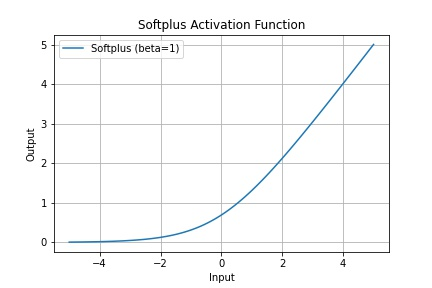
\includegraphics[width=9.5cm]{softplus.jpg}
                \end{tcolorbox}
                \begin{minted}[]{python}
def softplus(x, beta):
    # log(1+exp(B*x)) = log(1+exp(B*x)) - log(exp(B*x)) + 
    # B*x = log(1+exp(-B*x)) + B*x
    data = [(math.log(1+math.exp(-abs(value*beta))) +
             max(value*beta, 0))/beta for value in x]
    return np.array(data, dtype=float) 
def derv_softplus(x, beta):
    # log(1+exp(-B*x)) + B*x -> dy/dx = (-B*exp(-B*x))/(1+exp(-B*x)) + B
    data = [-math.exp(-(value*beta))/(1+math.exp(-(value*beta))) + 1
              for value in x]
    return np.array(data, dtype=float)                 
                \end{minted}
          \item GELU
                \begin{tcolorbox}
                  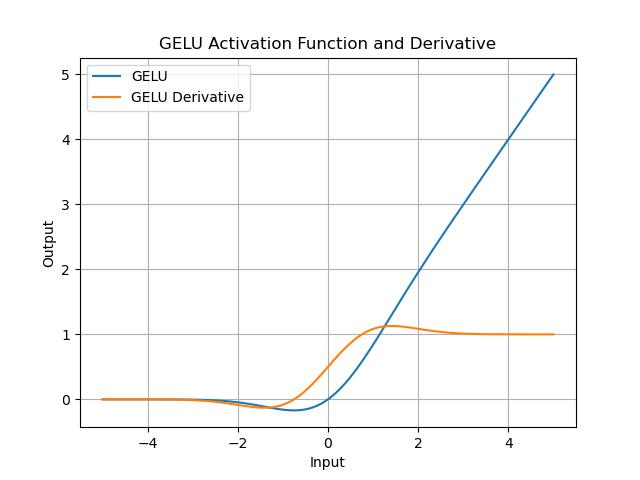
\includegraphics[width=9.5cm]{gelu.jpg}
                \end{tcolorbox}
                \begin{minted}[]{python}
from math import erf
def GELU(x):
    data = [0.5 * value * (1.0 + erf(value / np.sqrt(2.0))) for value in x]
    return np.array(data, dtype=float)  
def derv_GELU(x):
    data = [0.5*(1+erf(value / np.sqrt(2.0)))+
    value*math.exp((-value**2)/2)/np.sqrt(2*np.pi) for value in x]
    return np.array(data, dtype=float)                
                \end{minted}
        \end{enumerate}
  \item What are 4 different types of linear transformations? What is the
        role of linear transformation and non linear transformation in a neural
        network?
        \begin{tcolorbox}
          Reflection, rotation, scaling, and shear are the main types of
          linear transformations. In neural networks, each output unit produces the
          linear combination of the inputs and the connection weights. Once we allow
          translation, these essentially become affine transformations. To introduce
          nonlinearity to the model (to capture greater complexity by having a larger hypothesis space), activation functions ingest these transformations
          through a nonlinear function and treat that as the unit output.
        \end{tcolorbox}
  \item Given a neural network F parameterized by parameters $\theta$,
        denoted $F_\theta$, dataset $D = x_1, x_2,\ldots, x_N $, and labels $Y = y_1,
          y_2,\ldots, y_N$, write down the mathematical definition of training a neural
        network with the MSE loss function $\ell_{MSE}(\bm{\hat{y},y})=||\hat{y}-y||^2$
        \begin{tcolorbox}
          \begin{flalign*}
            F_\theta \impliedby \arg \min_{\theta}||F(D)-y||^2  
          \end{flalign*}
        \end{tcolorbox}
\end{enumerate}

\section*{Implementation}
%
\subsection*{Backpropagation }
You need to implement the forward pass and backward pass for Linear, ReLU,
Sigmoid, MSE loss, and BCE loss in the attached mlp.py file. We provide three
example test cases test1.py, test2.py, test3.py. We will test your
implementation with other hidden test cases, so please create your own test
cases to make sure your implementation is correct.
\subsection*{Gradient Descent}
Given a image classifier, implement a function that performs optimization on
the input (the image), to find the image that most highly represents the class.
Extra credit awarded for cool visuals. See gd.py.

\end{document}